\documentclass[aspectratio=169,10pt]{beamer}
\usepackage[T1]{fontenc}
\usepackage{lmodern}
\usepackage[utf8]{inputenc}
\usepackage{amsmath,amssymb}
\usepackage{xcolor}
\usepackage{tikz}
\usepackage{array}
\usepackage{booktabs}
\usepackage{colortbl}
\usetikzlibrary{arrows.meta,positioning,shapes.geometric,calc,fit,
                decorations.pathreplacing,backgrounds}

% ---- Palette ----------------------------------------------------------------
\definecolor{maroon}{HTML}{800020}
\definecolor{maroondk}{HTML}{5C0017}
\definecolor{ink}{HTML}{1F1F1F}
\definecolor{muted}{HTML}{6B6B6B}
\definecolor{cardbg}{HTML}{F7F2F4}
\definecolor{cardbd}{HTML}{E4D5DA}
\definecolor{accentbg}{HTML}{FFF6E0}
\definecolor{accentbd}{HTML}{D6A02E}
\definecolor{good}{HTML}{2A6F2A}
\definecolor{warn}{HTML}{B83E2E}
\definecolor{sky}{HTML}{EAF1FA}
\definecolor{leaf}{HTML}{EAF5EA}
\definecolor{darkbg}{HTML}{0F1219}
\definecolor{darkpanel}{HTML}{21232F}
\definecolor{lighttext}{HTML}{E8E9EF}
\definecolor{bluelight}{HTML}{8DC6FF}
\definecolor{greenlight}{HTML}{72E882}
\definecolor{pinklight}{HTML}{FF8DA0}

% ---- Theme ------------------------------------------------------------------
\usetheme{default}
\setbeamertemplate{navigation symbols}{}
\setbeamercolor{frametitle}{fg=ink}
\setbeamerfont{frametitle}{series=\bfseries,size=\Large}
\setbeamercolor{title}{fg=maroon}
\setbeamertemplate{frametitle}{%
  \vspace{0.35cm}\hspace{0.5cm}{\insertframetitle}\par
  \vspace{-0.18cm}\hspace{0.5cm}{\color{maroon}\rule{4.2cm}{1.6pt}}%
}
\setbeamertemplate{footline}{%
  \begin{tikzpicture}[overlay,remember picture]
    \fill[maroon](current page.south west)
      rectangle([yshift=0.6cm]current page.south east);
    \node[anchor=south west,white,font=\small]
      at([xshift=0.4cm,yshift=0.13cm]current page.south west)
      {SafeCharge: BMS Digital Twin --- Group 6};
    \node[anchor=south east,white,font=\small]
      at([xshift=-0.4cm,yshift=0.13cm]current page.south east)
      {\insertframenumber};
  \end{tikzpicture}%
}
\tikzset{
  card/.style={draw=cardbd,fill=cardbg,rounded corners=3pt,
               line width=0.5pt,inner sep=5pt},
  callout/.style={draw=accentbd,fill=accentbg,line width=1pt,
                  rounded corners=3pt,inner sep=6pt},
  arrowstrong/.style={-{Stealth[length=4mm,width=3mm]},line width=1.3pt,maroon},
  arrowthin/.style={-{Stealth[length=2.5mm]},line width=0.7pt,muted},
  arrowblue/.style={-{Stealth[length=3.5mm,width=2.8mm]},line width=1.2pt,
                    blue!70!black},
}
\title{SafeCharge: Interactive BMS Digital Twin}
\author{Group 6}
\institute{Digital Engineering Summer Semester 2026 \textbar\
  Otto-von-Guericke-University Magdeburg}
\date{Sprint 2 --- May 2026}

\begin{document}

% =============================================================================
% 1 TITLE
% =============================================================================
\begin{frame}[plain]
\begin{tikzpicture}[overlay,remember picture]
  \fill[maroon](current page.north west)
    rectangle([xshift=0.42cm]current page.south west);
  \fill[maroon!15](current page.north east)
    rectangle([xshift=-3.5cm,yshift=-\paperheight]current page.north east);
\end{tikzpicture}
\vspace{0.8cm}
\begin{center}
  {\color{maroon}\bfseries\Huge SafeCharge}\\[0.2cm]
  {\bfseries\Large Interactive BMS Digital Twin}\\[0.4cm]
  {\color{maroon}\rule{2.5cm}{2pt}}\\[0.4cm]
  {\bfseries\large Group 6}\\[0.15cm]
  {\color{muted}\normalsize Digital Engineering \textbar\
   Otto-von-Guericke-University Magdeburg}\\[0.4cm]
  {\color{maroon}\bfseries\large Sprint 2 --- Full Implementation Update}\\[0.2cm]
  {\color{muted}\itshape\small May 2026 \quad\textbar\quad
   Live Unity demo running end-to-end}
\end{center}
\end{frame}

% =============================================================================
% 2 SPRINT JOURNEY
% =============================================================================
\begin{frame}{From Sprint 1 to Sprint 2}
\centering
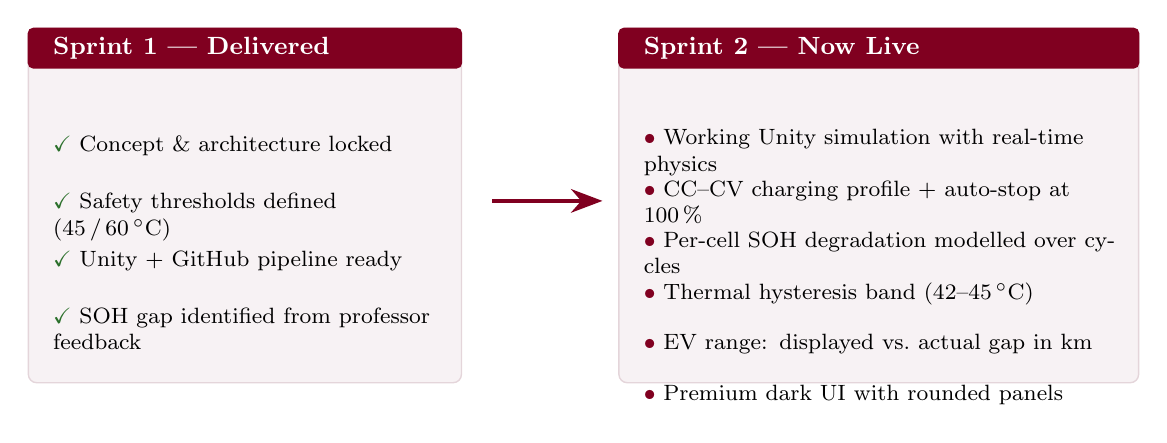
\begin{tikzpicture}
  \node[card,minimum width=5.5cm,minimum height=4.5cm,anchor=north west]
    (s1)at(0,0){};
  \fill[maroon,rounded corners=2pt](s1.north west)
    rectangle([yshift=-0.52cm]s1.north east);
  \node[anchor=west,white,font=\small\bfseries]
    at([xshift=0.2cm,yshift=-0.26cm]s1.north west){Sprint 1 --- Delivered};
  \foreach \i/\t in {
    1/{Concept \& architecture locked},
    2/{Safety thresholds defined (45\,/\,60\,$^\circ$C)},
    3/{Unity + GitHub pipeline ready},
    4/{SOH gap identified from professor feedback}
  }{
    \pgfmathparse{-0.52-\i*0.73}
    \node[anchor=north west,font=\footnotesize,text width=5.0cm]
      at([xshift=0.2cm,yshift=\pgfmathresult cm]s1.north west)
      {{\color{good}$\checkmark$}~\t};
  }
  \draw[arrowstrong](5.9,-2.2)--(7.3,-2.2);
  \node[card,minimum width=6.6cm,minimum height=4.5cm,anchor=north west]
    (s2)at(7.5,0){};
  \fill[maroon,rounded corners=2pt](s2.north west)
    rectangle([yshift=-0.52cm]s2.north east);
  \node[anchor=west,white,font=\small\bfseries]
    at([xshift=0.2cm,yshift=-0.26cm]s2.north west){Sprint 2 --- Now Live};
  \foreach \i/\t in {
    1/{Working Unity simulation with real-time physics},
    2/{CC--CV charging profile + auto-stop at 100\,\%},
    3/{Per-cell SOH degradation modelled over cycles},
    4/{Thermal hysteresis band (42--45\,$^\circ$C)},
    5/{EV range: displayed vs.\ actual gap in km},
    6/{Premium dark UI with rounded panels}
  }{
    \pgfmathparse{-0.52-\i*0.65}
    \node[anchor=north west,font=\footnotesize,text width=6.1cm]
      at([xshift=0.2cm,yshift=\pgfmathresult cm]s2.north west)
      {{\color{maroon}$\bullet$}~\t};
  }
\end{tikzpicture}
\end{frame}

% =============================================================================
% 3 PROFESSOR FEEDBACK
% =============================================================================
\begin{frame}{Professor's Feedback --- What the Gauge Hides}
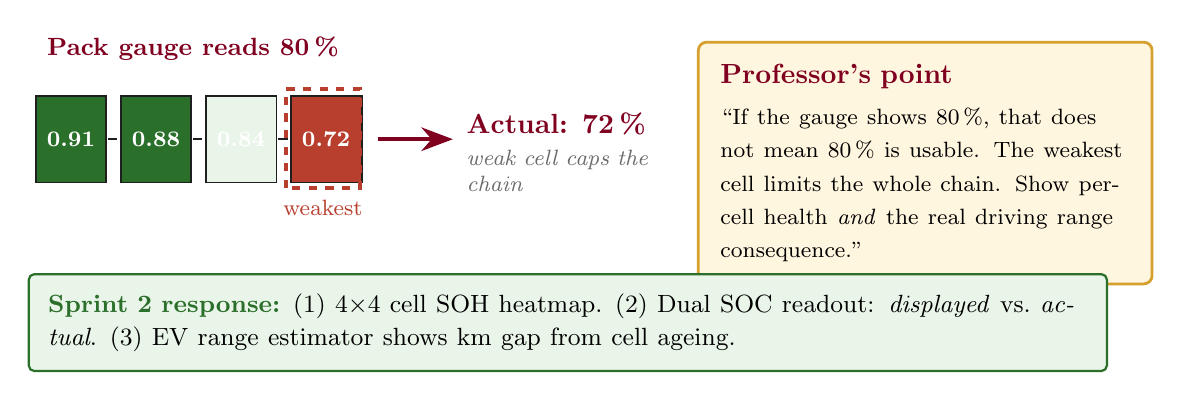
\begin{tikzpicture}
  \node[font=\small\bfseries,maroon]at(2.1,2.55){Pack gauge reads \textbf{80\,\%}};
  \foreach \i/\soh/\fc in {
    0/0.91/good, 1/0.88/good, 2/0.84/leaf, 3/0.72/warn%
  }{
    \node[draw=ink,fill=\fc,line width=0.7pt,minimum width=0.9cm,
          minimum height=1.1cm,font=\footnotesize\bfseries,text=white]
      at(\i*1.08+0.55,1.4){\soh};
  }
  \foreach \i in {0,1,2}{
    \draw[ink,line width=0.6pt](\i*1.08+1.02,1.4)--(\i*1.08+1.14,1.4);
  }
  \draw[warn,line width=1.3pt,dashed](3.28,0.78)rectangle(4.22,2.04);
  \node[font=\footnotesize,warn,anchor=north]at(3.75,0.75){weakest};
  \draw[arrowstrong](4.45,1.4)--(5.4,1.4);
  \node[font=\bfseries,maroon,anchor=west]at(5.45,1.6){Actual: 72\,\%};
  \node[font=\footnotesize\itshape,muted,anchor=west,text width=2.8cm]
    at(5.45,1.0){weak cell caps the chain};
  \node[callout,anchor=north west,text width=5.2cm,inner sep=8pt]
    at(8.5,2.65){%
    \textbf{\color{maroon}Professor's point}\\[0.1cm]
    \footnotesize
    ``If the gauge shows 80\,\%, that does not mean 80\,\%
    is usable. The weakest cell limits the whole chain.
    Show per-cell health \emph{and} the real driving
    range consequence.''};
  \node[draw=good,fill=leaf,line width=0.8pt,rounded corners=2pt,
        text width=13.2cm,inner sep=7pt,anchor=north west]
    at(0.0,-0.3){%
    \small\textbf{\color{good}Sprint 2 response:}\enspace
    (1)~4$\times$4 cell SOH heatmap.\enspace
    (2)~Dual SOC readout: \emph{displayed} vs.\ \emph{actual}.\enspace
    (3)~EV range estimator shows km gap from cell ageing.};
\end{tikzpicture}
\end{frame}

% =============================================================================
% 4 FEATURE OVERVIEW  (header-bar card layout — no overlap)
% =============================================================================
\begin{frame}{Sprint 2 --- Feature Overview}
\centering
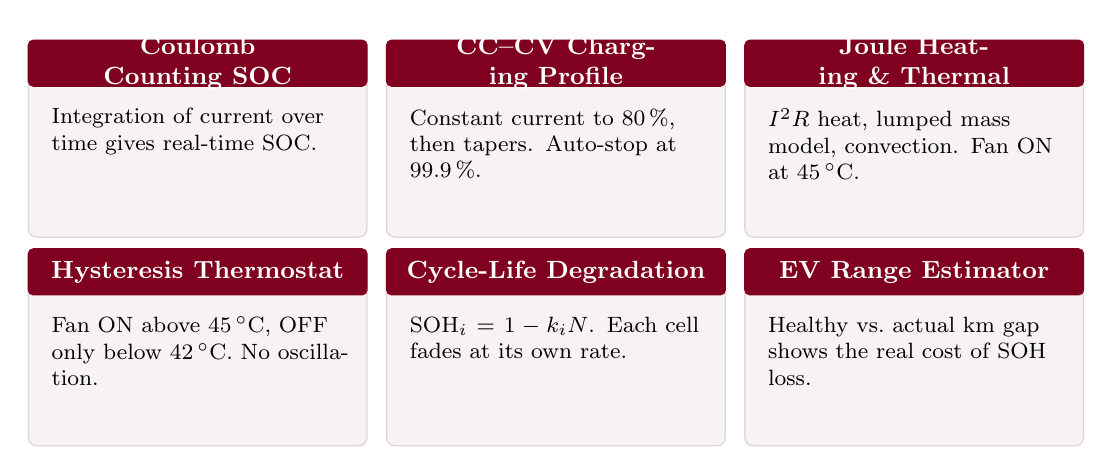
\begin{tikzpicture}
  \foreach \i/\ttl/\bdy in {%
    0/{Coulomb Counting SOC}/%
      {Integration of current over time gives real-time SOC.},%
    1/{CC--CV Charging Profile}/%
      {Constant current to 80\,\%, then tapers. Auto-stop at 99.9\,\%.},%
    2/{Joule Heating \& Thermal}/%
      {$I^2R$ heat, lumped mass model, convection. Fan ON at 45\,$^\circ$C.},%
    3/{Hysteresis Thermostat}/%
      {Fan ON above 45\,$^\circ$C, OFF only below 42\,$^\circ$C. No oscillation.},%
    4/{Cycle-Life Degradation}/%
      {$\text{SOH}_i = 1 - k_i N$. Each cell fades at its own rate.},%
    5/{EV Range Estimator}/%
      {Healthy vs.\ actual km gap shows the real cost of SOH loss.}%
  }{%
    \pgfmathtruncatemacro{\col}{mod(\i,3)}
    \pgfmathtruncatemacro{\row}{int(\i/3)}
    \begin{scope}[xshift=\col*4.55cm,yshift=-\row*2.65cm]
      % card body
      \node[card,minimum width=4.3cm,minimum height=2.5cm,anchor=north west]
        (g\i)at(0,0){};
      % maroon header bar — title centred, no icon
      \fill[maroon,rounded corners=2pt]
        (g\i.north west) rectangle ([yshift=-0.60cm]g\i.north east);
      \node[anchor=center,white,font=\small\bfseries,
            text width=3.9cm,align=center]
        at([yshift=-0.30cm]g\i.north){\ttl};
      % body text below header
      \node[anchor=north west,font=\footnotesize,text width=3.9cm]
        at([xshift=0.18cm,yshift=-0.75cm]g\i.north west){\bdy};
    \end{scope}
  }
\end{tikzpicture}
\end{frame}

% =============================================================================
% 5 SOC  (app convention: I > 0 = charging, I < 0 = discharging)
% =============================================================================
\begin{frame}{State of Charge --- Coulomb Counting}
\centering
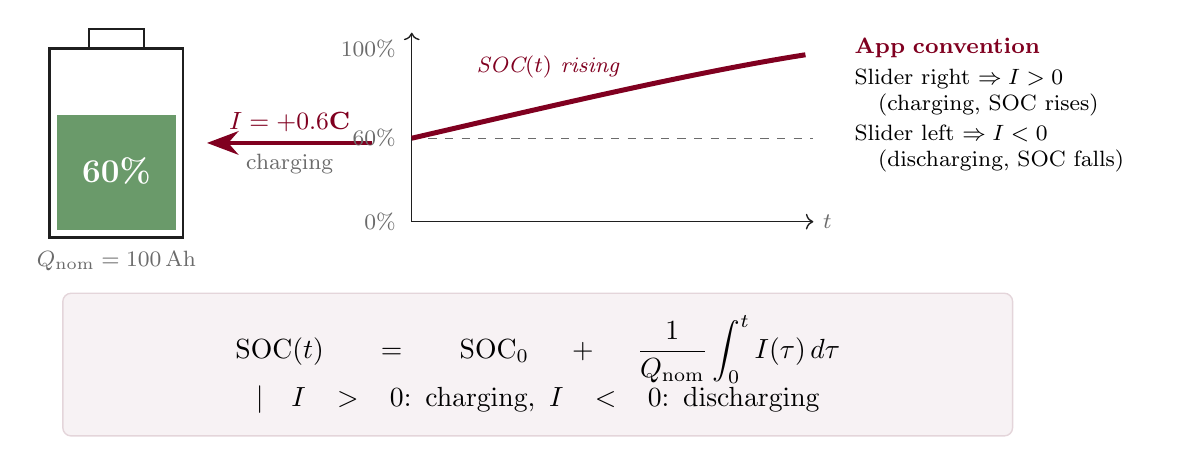
\begin{tikzpicture}
  % Battery at 60%, charging up
  \draw[ink,line width=0.8pt](0,0)rectangle(1.7,2.4);
  \draw[ink,line width=0.8pt](0.5,2.4)rectangle(1.2,2.65);
  \fill[good!70](0.1,0.1)rectangle(1.6,1.55);
  \node[font=\large\bfseries,white]at(0.85,0.85){60\%};
  \node[font=\footnotesize,muted,anchor=north]at(0.85,-0.05)
    {$Q_{\rm nom}=100$\,Ah};

  % Charging arrow (pointing IN to battery)
  \draw[arrowstrong](4.1,1.2)--(2.0,1.2)
    node[midway,above,maroon,font=\small\bfseries]{$I = +0.6$C}
    node[midway,below,muted,font=\footnotesize]{charging};

  % SOC rising curve
  \draw[ink,line width=0.5pt,->](4.6,0.2)--(4.6,2.6);
  \draw[ink,line width=0.5pt,->](4.6,0.2)--(9.7,0.2)
    node[right,font=\footnotesize,muted]{$t$};
  \node[anchor=east,font=\footnotesize,muted]at(4.52,2.4){100\%};
  \node[anchor=east,font=\footnotesize,muted]at(4.52,1.26){60\%};
  \node[anchor=east,font=\footnotesize,muted]at(4.52,0.2){0\%};
  \draw[muted,dashed,line width=0.5pt](4.6,1.26)--(9.7,1.26);
  \draw[maroon,line width=1.8pt](4.6,1.26)
    .. controls (6.5,1.7) and (8.2,2.1) .. (9.6,2.32);
  \node[font=\footnotesize\itshape,maroon,anchor=south west]at(5.3,1.9)
    {SOC$(t)$ rising};

  % Equation box
  \node[card,anchor=north,text width=11.5cm,inner sep=8pt,align=center]
    at(6.2,-0.7){%
    $\displaystyle
    \mathrm{SOC}(t) \;=\; \mathrm{SOC}_0
    \;+\;\frac{1}{Q_{\mathrm{nom}}}\int_0^t I(\tau)\,d\tau$
    \quad\textbar\quad
    $I > 0$: charging,\enspace $I < 0$: discharging};

  % Convention note
  \node[anchor=north west,font=\footnotesize,text width=3.8cm]
    at(10.1,2.65){%
    \textbf{\color{maroon}App convention}\\[0.05cm]
    Slider right $\Rightarrow I>0$\\
    \quad (charging, SOC rises)\\[0.05cm]
    Slider left $\Rightarrow I<0$\\
    \quad (discharging, SOC falls)};
\end{tikzpicture}

\vspace{0.0cm}
{\color{muted}\itshape\footnotesize
Implemented as $\Delta\mathrm{SOC} = I\,\Delta t / Q_{\rm nom}$ every physics step.
Source: Plett (2015), BMS Vol.\,I.}
\end{frame}

% =============================================================================
% 6 CC-CV  (all Bezier curves use explicit controls — no \tikz@curveto@auto)
% =============================================================================
\begin{frame}{CC--CV Charging Profile}
\centering
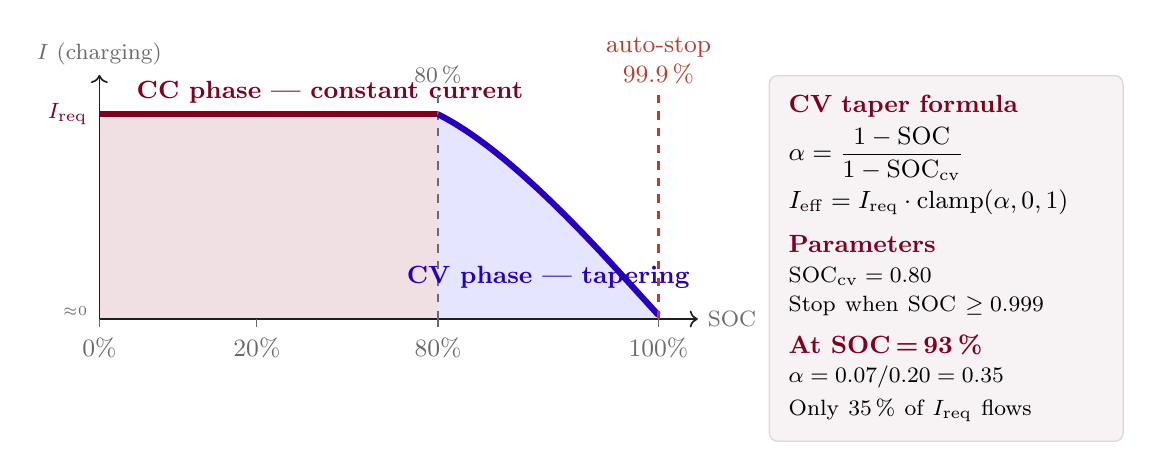
\begin{tikzpicture}
  % Compressed graph: 0% at x=0.5, 80% at x=4.8, 100% at x=7.6
  \fill[maroon!12](0.5,0.4)rectangle(4.8,3.0);
  \fill[blue!10]
    (4.8,0.4)--(4.8,3.0)
    .. controls (5.8,2.5) and (7.0,1.1) .. (7.6,0.45)
    --(7.6,0.4)--cycle;

  % Axes
  \draw[ink,line width=0.6pt,->](0.5,0.4)--(8.1,0.4)
    node[right,font=\footnotesize,muted]{SOC};
  \draw[ink,line width=0.6pt,->](0.5,0.4)--(0.5,3.5)
    node[above,font=\footnotesize,muted]{$I$ (charging)};

  % SOC ticks
  \foreach \x/\lbl in {0.5/{0\%},2.5/{20\%},4.8/{80\%},7.6/{100\%}}{
    \draw[muted,line width=0.4pt](\x,0.4)--(\x,0.3);
    \node[anchor=north,font=\small,muted]at(\x,0.28){\lbl};
  }
  \node[anchor=east,font=\footnotesize,maroon]at(0.47,3.0){$I_{\rm req}$};
  \node[anchor=east,font=\tiny,muted]at(0.47,0.5){${\approx}0$};

  % CC phase
  \draw[maroon,line width=2.2pt](0.5,3.0)--(4.8,3.0);
  \node[font=\small\bfseries,maroon,anchor=south west]at(0.85,3.02)
    {\textbf{CC phase} --- constant current};

  % CC/CV threshold dashed line
  \draw[muted,dashed,line width=0.8pt](4.8,0.4)--(4.8,3.25);
  \node[font=\footnotesize,muted,anchor=south]at(4.8,3.26){80\,\%};

  % CV taper
  \draw[blue!70!maroon,line width=2.2pt]
    (4.8,3.0) .. controls (5.8,2.5) and (7.0,1.1) .. (7.6,0.45);
  % Label placed ABOVE the curve (anchor=south so text grows upward from y=3.10)
  % Label at centre of blue region; bezier at x=6.2 has y≈1.93, so y=1.20 is 0.7cm clear
  \node[font=\small\bfseries,blue!70!maroon,anchor=north]at(6.2,1.20)
    {\textbf{CV phase} --- tapering};

  % Auto-stop dashed line
  \draw[warn,dashed,line width=0.8pt](7.6,0.4)--(7.6,3.25);
  \node[font=\small,warn,anchor=south,align=center]at(7.6,3.26)
    {auto-stop \\ 99.9\,\%};

  % Formula card — shifted right to clear the SOC axis label
  \node[card,anchor=north west,text width=4.0cm,inner sep=7pt]
    at(9.0,3.5){%
    \small\textbf{\color{maroon}CV taper formula}\\[0.1cm]
    $\displaystyle\alpha =
      \frac{1-\mathrm{SOC}}{1-\mathrm{SOC_{cv}}}$\\[0.08cm]
    $I_{\rm eff} = I_{\rm req}\cdot\mathrm{clamp}(\alpha,0,1)$\\[0.18cm]
    \small\textbf{\color{maroon}Parameters}\\[0.04cm]
    \footnotesize
    $\mathrm{SOC_{cv}} = 0.80$\\[0.04cm]
    Stop when SOC $\geq 0.999$\\[0.14cm]
    \small\textbf{\color{maroon}At SOC\,=\,93\,\%}\\[0.04cm]
    \footnotesize
    $\alpha = 0.07/0.20 = 0.35$\\
    Only 35\,\% of $I_{\rm req}$ flows};
\end{tikzpicture}
\end{frame}

% =============================================================================
% 7 THERMAL MODEL
% =============================================================================
\begin{frame}{Joule Heating \& Lumped Thermal Model}
\centering
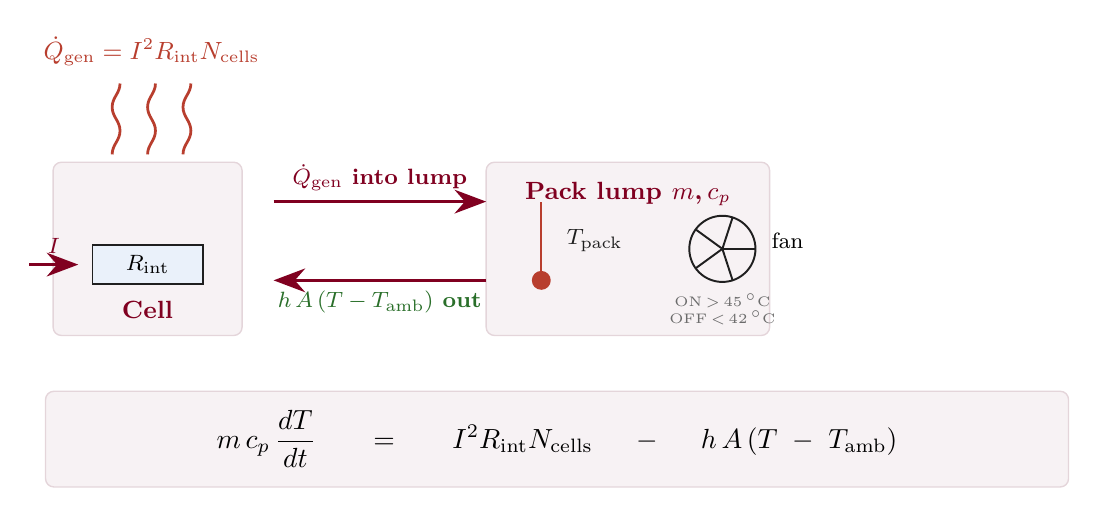
\begin{tikzpicture}
  \node[card,minimum width=2.4cm,minimum height=2.2cm](cell)at(1.3,1.3){};
  \node[draw=ink,fill=sky,line width=0.6pt,minimum width=1.4cm,
        minimum height=0.5cm,font=\footnotesize](R)at(1.3,1.1){$R_{\rm int}$};
  \node[font=\small\bfseries,maroon,anchor=south]
    at($(cell.south)+(0,0.1)$){Cell};
  \draw[arrowstrong](-0.2,1.1)--(0.42,1.1)
    node[midway,above,font=\footnotesize,maroon]{$I$};
  \foreach \dx in {-0.45,0,0.45}{
    \draw[warn,line width=1.0pt]($(1.3+\dx,2.5)$)
      to[out=90,in=270]($(1.4+\dx,2.8)$)
      to[out=90,in=270]($(1.3+\dx,3.1)$)
      to[out=90,in=270]($(1.4+\dx,3.4)$);
  }
  \node[font=\small\bfseries,warn,anchor=south]at(1.35,3.5)
    {$\dot{Q}_{\rm gen}=I^2 R_{\rm int} N_{\rm cells}$};
  \node[card,minimum width=3.6cm,minimum height=2.2cm](pack)at(7.4,1.3){};
  \node[font=\small\bfseries,maroon,anchor=north]
    at($(pack.north)+(0,-0.14)$){Pack lump $m$,\,$c_p$};
  \draw[warn,line width=0.7pt](6.3,0.9)--(6.3,1.9);
  \fill[warn](6.3,0.9)circle(0.12);
  \node[font=\footnotesize,anchor=west,ink]at(6.5,1.4){$T_{\rm pack}$};
  \draw[ink,line width=0.7pt](8.6,1.3)circle(0.42);
  \foreach \a in {0,72,144,216,288}{
    \draw[ink,line width=0.7pt](8.6,1.3)--++({\a}:0.42);
  }
  \node[font=\footnotesize,anchor=west]at(9.1,1.4){fan};
  \node[font=\tiny,muted,anchor=north,align=center]at(8.6,0.85)
    {ON\,$>$\,45\,$^\circ$C\\OFF\,$<$\,42\,$^\circ$C};
  \draw[arrowstrong](2.9,1.9)--(5.6,1.9)
    node[midway,above,font=\footnotesize\bfseries,maroon]
    {$\dot{Q}_{\rm gen}$ into lump};
  \draw[arrowstrong](5.6,0.9)--(2.9,0.9)
    node[midway,below,font=\footnotesize\bfseries,good]
    {$h\,A\,(T-T_{\rm amb})$ out};
  \node[card,text width=12.5cm,inner sep=7pt,align=center,anchor=north]
    at(6.5,-0.5){%
    $\displaystyle
    m\,c_p\,\frac{dT}{dt}
    \;=\; I^2 R_{\rm int} N_{\rm cells}
    \;-\; h\,A\,(T-T_{\rm amb})$};
\end{tikzpicture}
{\color{muted}\itshape\footnotesize
$h_{\rm passive}=10$\,W/m$^2$K,\;$h_{\rm active}=40$\,W/m$^2$K.\quad
Sources: Bernardi et al.\ (1985); Forgez et al.\ (2010).}
\end{frame}

% =============================================================================
% 8 THERMAL HYSTERESIS
% =============================================================================
\begin{frame}{Thermal Safety --- Hysteresis Thermostat}
\centering
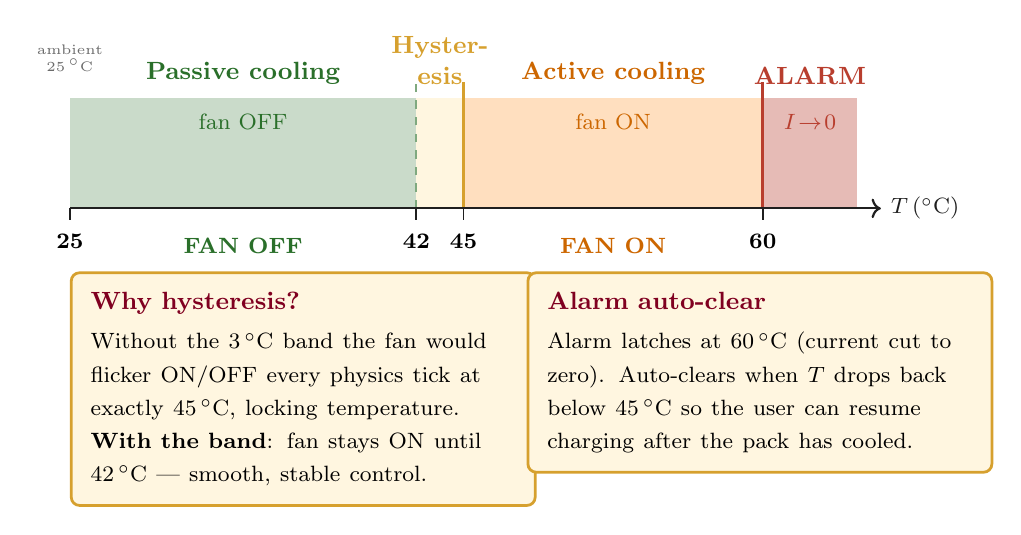
\begin{tikzpicture}
  % Colour zones
  \fill[good!25](0.0,1.6)rectangle(4.4,3.0);
  \fill[accentbg](4.4,1.6)rectangle(5.0,3.0);
  \fill[orange!25](5.0,1.6)rectangle(8.8,3.0);
  \fill[warn!35](8.8,1.6)rectangle(10.0,3.0);
  % Borders
  \draw[good!60,line width=0.6pt,dashed](4.4,1.6)--(4.4,3.2);
  \draw[accentbd,line width=1.0pt](5.0,1.6)--(5.0,3.2);
  \draw[warn,line width=1.0pt](8.8,1.6)--(8.8,3.2);
  % Axis
  \draw[ink,line width=0.8pt,->](0.0,1.6)--(10.3,1.6)
    node[right,font=\footnotesize]{$T$\,($^\circ$C)};
  % Ticks
  \foreach \x/\t in {0.0/25,4.4/42,5.0/45,8.8/60}{
    \draw[ink,line width=0.6pt](\x,1.6)--(\x,1.45);
    \node[anchor=north,font=\footnotesize\bfseries]at(\x,1.4){\t};
  }
  % Zone labels
  \node[font=\small\bfseries,good,anchor=south]at(2.2,3.05){Passive cooling};
  \node[font=\footnotesize,good]at(2.2,2.70){fan OFF};
  \node[font=\small\bfseries,accentbd,anchor=south,align=center]
    at(4.70,3.05){Hyster-\\esis};
  \node[font=\small\bfseries,orange!80!black,anchor=south]at(6.9,3.05)
    {Active cooling};
  \node[font=\footnotesize,orange!80!black]at(6.9,2.70){fan ON};
  \node[font=\small\bfseries,warn,anchor=south]at(9.4,3.05){ALARM};
  \node[font=\footnotesize,warn,align=center]at(9.4,2.70){$I\!\to\!0$};
  \node[font=\tiny,muted,anchor=south,align=center]at(0.0,3.22)
    {ambient\\25\,$^\circ$C};
  % State labels under axis
  \node[font=\footnotesize\bfseries,good,anchor=north]at(2.2,1.35){FAN OFF};
  \node[font=\footnotesize\bfseries,orange!80!black,anchor=north]at(6.9,1.35)
    {FAN ON};
  % Explanation boxes
  \node[callout,anchor=north west,text width=5.4cm,inner sep=7pt]
    at(0.0,0.8){%
    \small\textbf{\color{maroon}Why hysteresis?}\\[0.08cm]
    \footnotesize
    Without the 3\,$^\circ$C band the fan would flicker ON/OFF every
    physics tick at exactly 45\,$^\circ$C, locking temperature.
    \textbf{With the band}: fan stays ON until 42\,$^\circ$C ---
    smooth, stable control.};
  \node[callout,anchor=north west,text width=5.4cm,inner sep=7pt]
    at(5.8,0.8){%
    \small\textbf{\color{maroon}Alarm auto-clear}\\[0.08cm]
    \footnotesize
    Alarm latches at 60\,$^\circ$C (current cut to zero).
    Auto-clears when $T$ drops back below 45\,$^\circ$C so the
    user can resume charging after the pack has cooled.};
\end{tikzpicture}
\end{frame}

% =============================================================================
% 9 SOH & WEAKEST CELL
% =============================================================================
\begin{frame}{SOH \& the Weakest-Cell Rule}
\centering
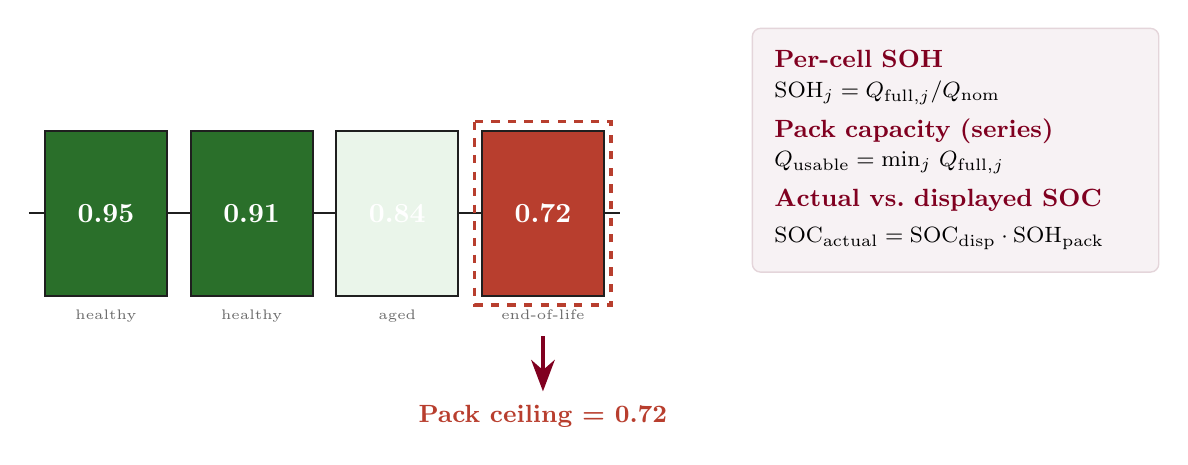
\begin{tikzpicture}
  \foreach \i/\soh/\col/\lbl in {
    0/0.95/good/{healthy},
    1/0.91/good/{healthy},
    2/0.84/leaf/{aged},
    3/0.72/warn/{end-of-life}
  }{
    \node[draw=ink,fill=\col,line width=0.7pt,minimum width=1.55cm,
          minimum height=2.1cm,text=white,font=\bfseries]
      (c\i)at(\i*1.85,0){\soh};
    \node[font=\tiny,anchor=north,muted,text width=1.7cm,align=center]
      at(\i*1.85,-1.1){\lbl};
  }
  \foreach \i in {0,1,2}{
    \pgfmathtruncatemacro{\j}{\i+1}
    \draw[ink,line width=0.8pt](\i*1.85+0.78,0)--(\j*1.85-0.78,0);
  }
  \draw[ink,line width=0.8pt](-0.98,0)--(-0.78,0);
  \draw[ink,line width=0.8pt](3*1.85+0.78,0)--(3*1.85+0.98,0);
  \draw[warn,dashed,line width=1.3pt]
    ($(c3.north west)+(-0.08,0.1)$)rectangle($(c3.south east)+(0.08,-0.1)$);
  \draw[arrowstrong](c3.south)++(0,-0.5)--++(0,-0.7);
  \node[font=\small\bfseries,warn,anchor=north]
    at($(c3.south)+(0,-1.25)$){Pack ceiling = 0.72};
  \node[card,anchor=west,text width=4.6cm,align=left,inner sep=8pt]
    at(8.2,0.8){%
    \small\textbf{\color{maroon}Per-cell SOH}\\[0.04cm]
    \footnotesize$\mathrm{SOH}_j = Q_{{\rm full},j} / Q_{\rm nom}$\\[0.12cm]
    \small\textbf{\color{maroon}Pack capacity (series)}\\[0.04cm]
    \footnotesize$Q_{\rm usable} = \min_j\,Q_{{\rm full},j}$\\[0.12cm]
    \small\textbf{\color{maroon}Actual vs.\ displayed SOC}\\[0.04cm]
    \footnotesize$\mathrm{SOC}_{\rm actual}
      = \mathrm{SOC}_{\rm disp}\cdot\mathrm{SOH}_{\rm pack}$};
\end{tikzpicture}
{\color{muted}\itshape\footnotesize
Cells in series: the weakest link sets the pack limit.
Sources: Dubarry et al.\ (2009); IEC 62660-1:2018.}
\end{frame}

% =============================================================================
% 10 CYCLE DEGRADATION  (clearer labels with filled boxes)
% =============================================================================
\begin{frame}{Cycle-Life Degradation Model}
\centering
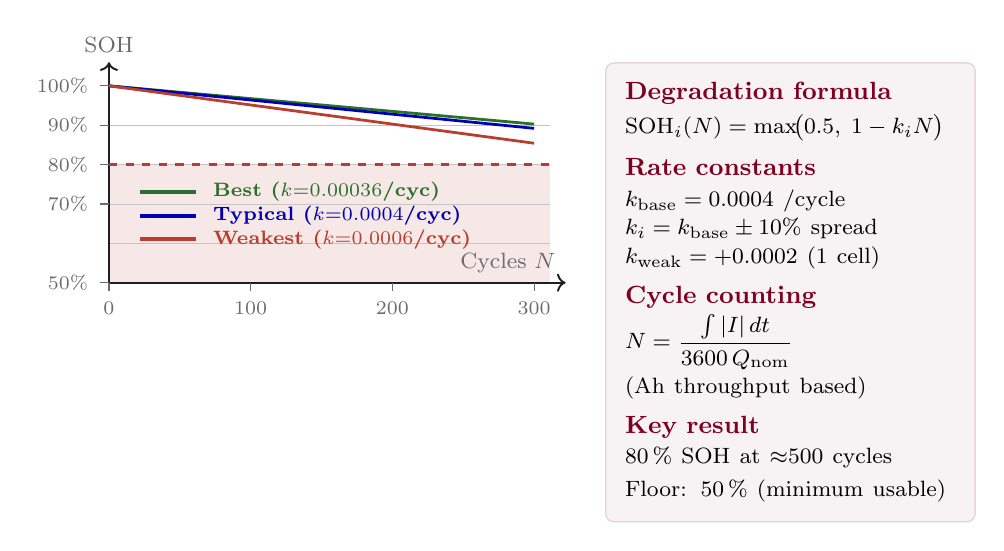
\begin{tikzpicture}
  % y: SOH mapped as y=(SOH-0.5)*5  => SOH=1.0->y=2.5, SOH=0.8->y=1.5, SOH=0.5->y=0
  % x: N/50 => x=9 means N=450 cycles

  % EOL shaded region — compressed to 300 cycles (x=5.4)
  \fill[warn!12](0.0,0.0)rectangle(5.6,1.5);

  % Gridlines
  \foreach \y in {0.5,1.0,1.5,2.0}{
    \draw[muted!40,line width=0.3pt](0.0,\y)--(5.6,\y);
  }

  % Axes
  \draw[ink,line width=0.7pt,->](0,0)--(0,2.8)
    node[above,font=\footnotesize,muted]{SOH};
  \draw[ink,line width=0.7pt,->](0,0)--(5.8,0)
    node[pos=1,above left,font=\footnotesize,muted]{Cycles $N$};

  % Y-axis labels
  \foreach \y/\lbl in {0.0/{50\%},1.0/{70\%},1.5/{80\%},2.0/{90\%},2.5/{100\%}}{
    \draw[muted,line width=0.4pt](-0.12,\y)--(0,\y);
    \node[anchor=east,font=\scriptsize,muted]at(-0.14,\y){\lbl};
  }
  % X-axis labels: 0–300 cycles
  \foreach \x/\lbl in {0/0,1.8/100,3.6/200,5.4/300}{
    \draw[muted,line width=0.4pt](\x,-0.1)--(\x,0);
    \node[anchor=north,font=\scriptsize,muted]at(\x,-0.12){\lbl};
  }

  % EOL dashed line at 80% SOH
  \draw[warn,dashed,line width=0.9pt](0,1.5)--(5.6,1.5);

  % Data lines to x=5.4 (300 cycles); same slopes as original
  % Best:    2.5 - 0.09*5.4 = 2.014
  \draw[good,line width=1.0pt](0,2.5)--(5.4,2.014);
  % Typical: 2.5 - 0.10*5.4 = 1.960
  \draw[blue!70!black,line width=1.0pt](0,2.5)--(5.4,1.960);
  % Weakest: 2.5 - 0.135*5.4 = 1.771
  \draw[warn,line width=1.0pt](0,2.5)--(5.4,1.771);

  % Legend — inside the shaded zone (below 80% SOH), data lines never reach here
  \draw[good,line width=1.5pt](0.4,1.15)--(1.1,1.15);
  \node[anchor=west,font=\scriptsize\bfseries,good]at(1.2,1.15)
    {Best ($k{=}0.00036$/cyc)};
  \draw[blue!70!black,line width=1.5pt](0.4,0.85)--(1.1,0.85);
  \node[anchor=west,font=\scriptsize\bfseries,blue!70!black]at(1.2,0.85)
    {Typical ($k{=}0.0004$/cyc)};
  \draw[warn,line width=1.5pt](0.4,0.55)--(1.1,0.55);
  \node[anchor=west,font=\scriptsize\bfseries,warn]at(1.2,0.55)
    {Weakest ($k{=}0.0006$/cyc)};

  % Formula card — comfortably right of compressed graph
  \node[card,anchor=north west,text width=4.2cm,inner sep=7pt]
    at(6.3,2.8){%
    \small\textbf{\color{maroon}Degradation formula}\\[0.1cm]
    \footnotesize
    $\mathrm{SOH}_i(N)=\max\!\bigl(0.5,\;1-k_i N\bigr)$\\[0.15cm]
    \small\textbf{\color{maroon}Rate constants}\\[0.05cm]
    \footnotesize
    $k_{\rm base}= 0.0004$ /cycle\\[0.03cm]
    $k_i = k_{\rm base}\pm10\%$ spread\\[0.03cm]
    $k_{\rm weak}= +0.0002$ (1 cell)\\[0.12cm]
    \small\textbf{\color{maroon}Cycle counting}\\[0.05cm]
    \footnotesize
    $\displaystyle N = \frac{\int|I|\,dt}{3600\,Q_{\rm nom}}$\\[0.06cm]
    (Ah throughput based)\\[0.12cm]
    \small\textbf{\color{maroon}Key result}\\[0.05cm]
    \footnotesize
    80\,\% SOH at ${\approx}500$ cycles\\
    Floor: 50\,\% (minimum usable)};
\end{tikzpicture}
\end{frame}

% =============================================================================
% 11 EV RANGE
% =============================================================================
\begin{frame}{EV Range --- Closing the Gap}
\centering
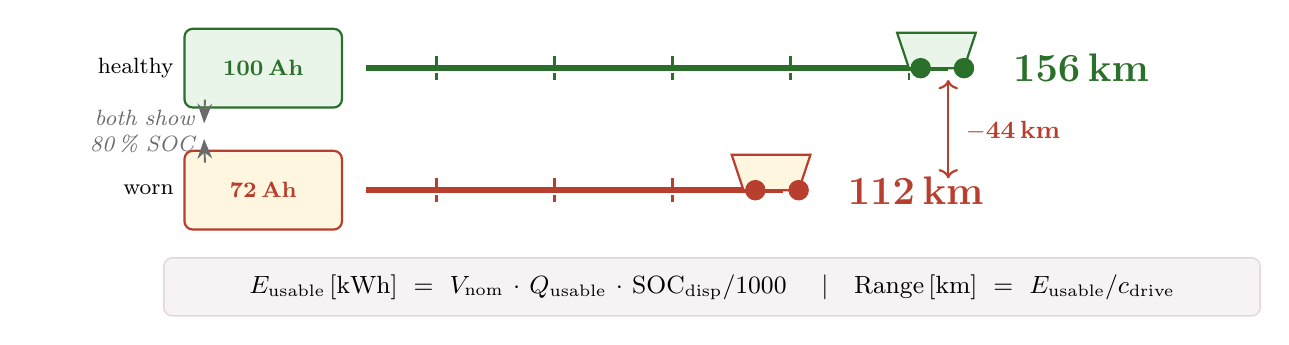
\begin{tikzpicture}
  % Healthy row
  \node[card,minimum width=2.0cm,minimum height=1.0cm,
        fill=leaf,draw=good,line width=0.8pt](hp)at(0.8,1.9){};
  \node[font=\footnotesize\bfseries,good]at(hp.center){100\,Ah};
  \node[font=\footnotesize,anchor=east]at(hp.west){healthy};
  \draw[good,line width=2pt](2.1,1.9)--(9.5,1.9);
  \foreach \x in {3.0,4.5,6.0,7.5,9.0}{
    \draw[good,dashed,line width=1pt](\x,2.05)--(\x,1.75);}
  \draw[good,fill=leaf,line width=0.8pt]
    (9.0,1.9)--++(0.7,0)--++(0.15,0.45)--++(-1.0,0)--++(0.15,-0.45);
  \fill[good](9.15,1.9)circle(0.13);
  \fill[good](9.7,1.9)circle(0.13);
  \node[font=\Large\bfseries,good,anchor=west]at(10.2,1.9){156\,km};
  % Worn row
  \node[card,minimum width=2.0cm,minimum height=1.0cm,
        fill=accentbg,draw=warn,line width=0.8pt](wp)at(0.8,0.35){};
  \node[font=\footnotesize\bfseries,warn]at(wp.center){72\,Ah};
  \node[font=\footnotesize,anchor=east]at(wp.west){worn};
  \draw[warn,line width=2pt](2.1,0.35)--(7.4,0.35);
  \foreach \x in {3.0,4.5,6.0}{
    \draw[warn,dashed,line width=1pt](\x,0.5)--(\x,0.2);}
  \draw[warn,fill=accentbg,line width=0.8pt]
    (6.9,0.35)--++(0.7,0)--++(0.15,0.45)--++(-1.0,0)--++(0.15,-0.45);
  \fill[warn](7.05,0.35)circle(0.13);
  \fill[warn](7.6,0.35)circle(0.13);
  \node[font=\Large\bfseries,warn,anchor=west]at(8.1,0.35){112\,km};
  % Common SOC note
  \node[anchor=east,font=\footnotesize\itshape,muted,text width=2.0cm,align=right]
    at(0.05,1.1){both show\\80\,\% SOC};
  \draw[arrowthin](0.06,1.5)--(0.05,1.2);
  \draw[arrowthin](0.06,0.7)--(0.05,1.0);
  % Delta bracket
  \draw[warn,<->,line width=0.8pt](9.5,0.5)--(9.5,1.75);
  \node[font=\small\bfseries,warn,anchor=west]at(9.6,1.1){$-$44\,km};
  % Equations
  \node[card,text width=13.5cm,inner sep=6pt,align=center,anchor=north]
    at(6.5,-0.5){%
    \small
    $E_{\rm usable}\,[\mathrm{kWh}] = V_{\rm nom}\cdot Q_{\rm usable}
      \cdot \mathrm{SOC}_{\rm disp} / 1000$
    \quad$|$\quad
    $\mathrm{Range}\,[\mathrm{km}] = E_{\rm usable} / c_{\rm drive}$};
\end{tikzpicture}
{\color{muted}\itshape\footnotesize
$V_{\rm nom}=350$\,V,\;$Q_{\rm nom}=100$\,Ah,\;$c_{\rm drive}=0.18$\,kWh/km.
\quad Source: Larminie \& Lowry (2012).}
\end{frame}

% =============================================================================
% 12 DASHBOARD UI (dark theme mockup)
% =============================================================================
\begin{frame}{Dashboard UI --- Premium Dark Theme}
\centering
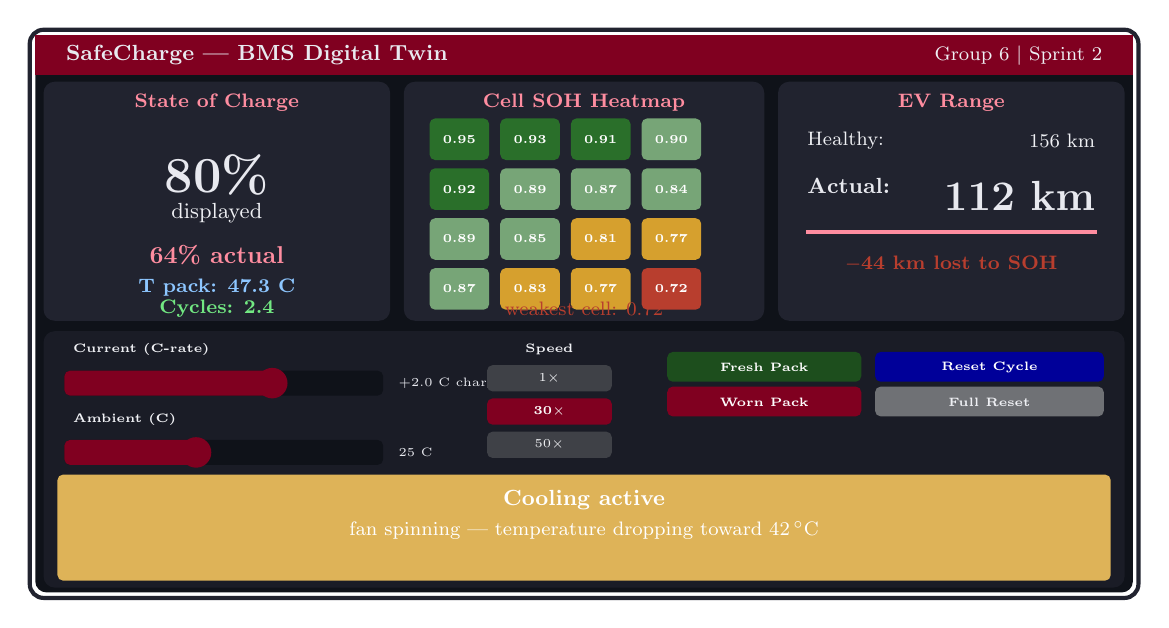
\begin{tikzpicture}[scale=0.88,transform shape]
  % Screen
  \draw[darkpanel,line width=1.5pt,rounded corners=5pt]
    (0,0)rectangle(16,8.2);
  \fill[darkbg,rounded corners=4pt](0.08,0.08)rectangle(15.92,8.12);
  % Top bar
  \fill[maroon](0.08,7.55)rectangle(15.92,8.12);
  \node[anchor=west,lighttext,font=\small\bfseries]at(0.4,7.83)
    {SafeCharge --- BMS Digital Twin};
  \node[anchor=east,lighttext!70,font=\footnotesize]at(15.6,7.83)
    {Group 6 \textbar\ Sprint 2};
  % SOC panel
  \fill[darkpanel,rounded corners=4pt](0.2,4.0)rectangle(5.2,7.45);
  \node[font=\footnotesize\bfseries,pinklight]at(2.7,7.15){State of Charge};
  \node[font=\fontsize{20}{20}\selectfont\bfseries,lighttext]at(2.7,6.1){80\%};
  \node[font=\small,lighttext!70]at(2.7,5.55){displayed};
  \node[font=\normalsize\bfseries,pinklight]at(2.7,4.95){64\% actual};
  \node[font=\footnotesize\bfseries,bluelight]at(2.7,4.48){T pack: 47.3 C};
  \node[font=\footnotesize\bfseries,greenlight]at(2.7,4.18){Cycles: 2.4};
  % Heatmap panel
  \fill[darkpanel,rounded corners=4pt](5.4,4.0)rectangle(10.6,7.45);
  \node[font=\footnotesize\bfseries,pinklight]at(8.0,7.15){Cell SOH Heatmap};
  \foreach \ci/\ri/\sohv/\fc in {
    0/0/0.95/good,   1/0/0.93/good,   2/0/0.91/good,   3/0/0.90/good!60!leaf,
    0/1/0.92/good,   1/1/0.89/good!60!leaf, 2/1/0.87/good!60!leaf, 3/1/0.84/good!60!leaf,
    0/2/0.89/good!60!leaf, 1/2/0.85/good!60!leaf, 2/2/0.81/accentbd, 3/2/0.77/accentbd,
    0/3/0.87/good!60!leaf, 1/3/0.83/accentbd, 2/3/0.77/accentbd, 3/3/0.72/warn%
  }{
    \pgfmathsetmacro{\xcc}{6.2+\ci*1.02}
    \pgfmathsetmacro{\ycc}{6.62-\ri*0.72}
    \fill[\fc,rounded corners=2pt](\xcc-0.43,\ycc-0.30)rectangle(\xcc+0.43,\ycc+0.30);
    \node[font=\tiny\bfseries,white]at(\xcc,\ycc){\sohv};
  }
  \node[font=\footnotesize,warn]at(8.0,4.18){weakest cell: 0.72};
  % Range panel
  \fill[darkpanel,rounded corners=4pt](10.8,4.0)rectangle(15.8,7.45);
  \node[font=\footnotesize\bfseries,pinklight]at(13.3,7.15){EV Range};
  \node[font=\footnotesize,lighttext!70,anchor=west]at(11.1,6.6){Healthy:};
  \node[font=\footnotesize,lighttext!70,anchor=east]at(15.5,6.6){156 km};
  \node[font=\small\bfseries,lighttext,anchor=west]at(11.1,5.95){Actual:};
  \node[font=\fontsize{18}{18}\selectfont\bfseries,lighttext,anchor=east]
    at(15.5,5.8){112 km};
  \draw[pinklight,line width=1.5pt](11.2,5.28)--(15.4,5.28);
  \node[font=\footnotesize\bfseries,warn]at(13.3,4.82)
    {$-$44 km lost to SOH};
  % Controls bar
  \fill[darkpanel!80!black,rounded corners=4pt](0.2,0.15)rectangle(15.8,3.85);
  \node[font=\tiny\bfseries,lighttext!70,anchor=west]at(0.5,3.58){Current (C-rate)};
  \fill[darkbg,rounded corners=2pt](0.5,2.92)rectangle(5.1,3.28);
  \fill[maroon,rounded corners=2pt](0.5,2.92)rectangle(3.5,3.28);
  \fill[maroon](3.5,3.10)circle(0.22);
  \node[font=\tiny,lighttext,anchor=west]at(5.2,3.10){$+$2.0 C charge};
  \node[font=\tiny\bfseries,lighttext!70,anchor=west]at(0.5,2.58){Ambient (C)};
  \fill[darkbg,rounded corners=2pt](0.5,1.92)rectangle(5.1,2.28);
  \fill[maroon,rounded corners=2pt](0.5,1.92)rectangle(2.4,2.28);
  \fill[maroon](2.4,2.10)circle(0.22);
  \node[font=\tiny,lighttext,anchor=west]at(5.2,2.10){25 C};
  \node[font=\tiny\bfseries,lighttext!70]at(7.5,3.58){Speed};
  \fill[darkbg!80,rounded corners=2pt](6.6,2.98)rectangle(8.4,3.36);
  \node[font=\tiny,lighttext!60]at(7.5,3.17){1$\times$};
  \fill[maroon,rounded corners=2pt](6.6,2.50)rectangle(8.4,2.88);
  \node[font=\tiny\bfseries,white]at(7.5,2.69){30$\times$};
  \fill[darkbg!80,rounded corners=2pt](6.6,2.02)rectangle(8.4,2.40);
  \node[font=\tiny,lighttext!60]at(7.5,2.21){50$\times$};
  \fill[good!70!black,rounded corners=2pt](9.2,3.12)rectangle(12.0,3.55);
  \node[font=\tiny\bfseries,white]at(10.6,3.33){Fresh Pack};
  \fill[maroon,rounded corners=2pt](9.2,2.62)rectangle(12.0,3.05);
  \node[font=\tiny\bfseries,white]at(10.6,2.83){Worn Pack};
  \fill[blue!60!black,rounded corners=2pt](12.2,3.12)rectangle(15.5,3.55);
  \node[font=\tiny\bfseries,white]at(13.85,3.33){Reset Cycle};
  \fill[darkbg!60,rounded corners=2pt](12.2,2.62)rectangle(15.5,3.05);
  \node[font=\tiny\bfseries,lighttext!70]at(13.85,2.83){Full Reset};
  \fill[accentbd!80,rounded corners=2pt](0.4,0.25)rectangle(15.6,1.78);
  \node[font=\small\bfseries,white]at(8.0,1.42){Cooling active};
  \node[font=\footnotesize,white!80]at(8.0,0.97)
    {fan spinning --- temperature dropping toward 42\,$^\circ$C};
\end{tikzpicture}
\end{frame}

% =============================================================================
% 13 BMS ARCHITECTURE  (star layout, all within frame, clean arrows)
% =============================================================================
\begin{frame}{BMS Software Architecture --- Event-Driven}
\centering
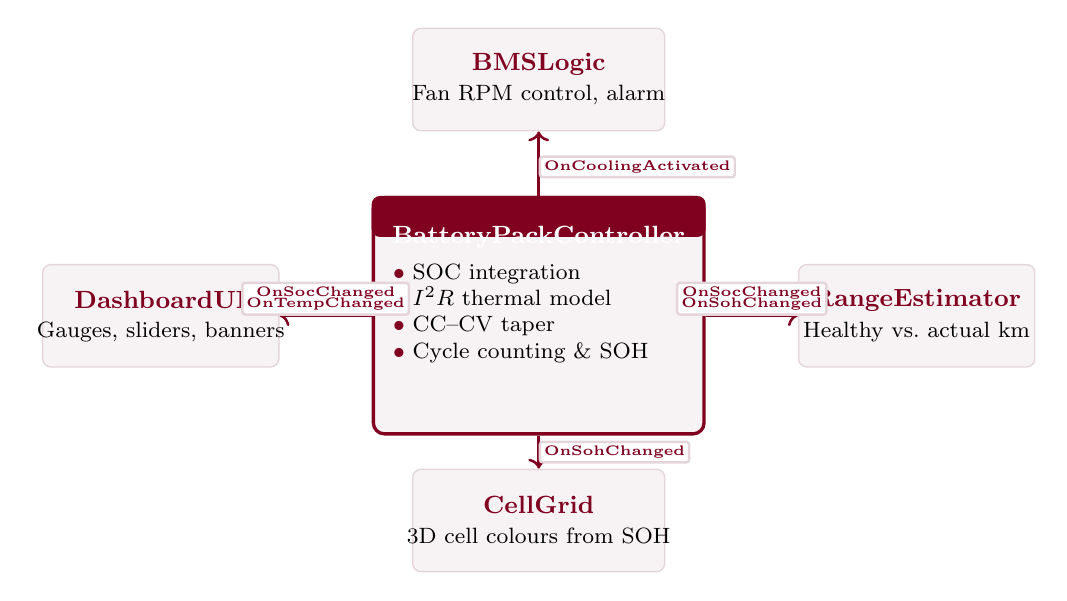
\begin{tikzpicture}
  % ---- Central controller ----
  \node[draw=maroon,fill=cardbg,line width=1.2pt,rounded corners=4pt,
        minimum width=4.2cm,minimum height=3.0cm]
    (ctrl)at(6.5,0){};
  \fill[maroon,rounded corners=3pt](ctrl.north west)
    rectangle([yshift=-0.52cm]ctrl.north east);
  \node[white,font=\small\bfseries,anchor=north]
    at([yshift=-0.26cm]ctrl.north){BatteryPackController};
  \node[font=\footnotesize,align=left,text width=3.7cm,anchor=north]
    at([yshift=-0.74cm]ctrl.north){%
    {\color{maroon}$\bullet$}~SOC integration\\
    {\color{maroon}$\bullet$}~$I^2R$ thermal model\\
    {\color{maroon}$\bullet$}~CC--CV taper\\
    {\color{maroon}$\bullet$}~Cycle counting \& SOH};

  % ---- Peripheral boxes ----
  \node[card,minimum width=3.2cm,minimum height=1.3cm]
    (bms)at(6.5,3.0){};
  \node[font=\small\bfseries,maroon,anchor=center]
    at([yshift=0.20cm]bms.center){BMSLogic};
  \node[font=\footnotesize,anchor=center]
    at([yshift=-0.20cm]bms.center){Fan RPM control, alarm};

  \node[card,minimum width=3.0cm,minimum height=1.3cm]
    (dash)at(1.7,0){};
  \node[font=\small\bfseries,maroon,anchor=center]
    at([yshift=0.20cm]dash.center){DashboardUI};
  \node[font=\footnotesize,anchor=center]
    at([yshift=-0.20cm]dash.center){Gauges, sliders, banners};

  \node[card,minimum width=3.0cm,minimum height=1.3cm]
    (range)at(11.3,0){};
  \node[font=\small\bfseries,maroon,anchor=center]
    at([yshift=0.20cm]range.center){RangeEstimator};
  \node[font=\footnotesize,anchor=center]
    at([yshift=-0.20cm]range.center){Healthy vs.\ actual km};

  \node[card,minimum width=3.2cm,minimum height=1.3cm]
    (grid)at(6.5,-2.6){};
  \node[font=\small\bfseries,maroon,anchor=center]
    at([yshift=0.20cm]grid.center){CellGrid};
  \node[font=\footnotesize,anchor=center]
    at([yshift=-0.20cm]grid.center){3D cell colours from SOH};

  % ---- Thin maroon arrows with inline event labels ----
  \draw[->,maroon,line width=0.9pt]
    (ctrl.north) -- node[pos=0.45,right,font=\tiny\bfseries,maroon,
      fill=white,draw=cardbd,rounded corners=1pt,inner sep=1.5pt]{OnCoolingActivated}
    (bms.south);

  \draw[->,maroon,line width=0.9pt]
    (ctrl.west) -- node[pos=0.5,above,font=\tiny\bfseries,maroon,
      fill=white,draw=cardbd,rounded corners=1pt,inner sep=1.5pt,align=center]
      {OnSocChanged\\[-2pt]OnTempChanged}
    (dash.east);

  \draw[->,maroon,line width=0.9pt]
    (ctrl.east) -- node[pos=0.5,above,font=\tiny\bfseries,maroon,
      fill=white,draw=cardbd,rounded corners=1pt,inner sep=1.5pt,align=center]
      {OnSocChanged\\[-2pt]OnSohChanged}
    (range.west);

  \draw[->,maroon,line width=0.9pt]
    (ctrl.south) -- node[pos=0.5,right,font=\tiny\bfseries,maroon,
      fill=white,draw=cardbd,rounded corners=1pt,inner sep=1.5pt]{OnSohChanged}
    (grid.north);
\end{tikzpicture}
\end{frame}

% =============================================================================
% 14 PARAMETERS  (two-column, all rows visible)
% =============================================================================
\begin{frame}{Model Parameters \& Assumptions}
\centering
\renewcommand{\arraystretch}{1.12}
\setlength{\arrayrulewidth}{0.4pt}
\setlength{\tabcolsep}{4pt}
\arrayrulecolor{cardbd}
{\footnotesize
\begin{tabular}{>{\bfseries\color{maroon}}m{1.3cm}
                >{\ttfamily\footnotesize}m{1.5cm}
                m{3.0cm}
                >{\bfseries\color{maroon}}m{1.3cm}
                >{\ttfamily\footnotesize}m{1.5cm}
                m{3.1cm}}
\arrayrulecolor{maroon}\toprule
\rowcolor{maroon}
\color{white}\textbf{Param.} &
\color{white}\textbf{Value} &
\color{white}\textbf{Meaning / Note} &
\color{white}\textbf{Param.} &
\color{white}\textbf{Value} &
\color{white}\textbf{Meaning / Note}\\
\arrayrulecolor{cardbd}\midrule
$Q_{\rm nom}$ & 100\,Ah & Pack nominal capacity &
$T_{\rm cool}$ & 45\,$^\circ$C & Fan trigger threshold\\
$V_{\rm nom}$ & 350\,V & Nominal pack voltage &
$T_{\rm hyst}$ & 42\,$^\circ$C & Fan OFF (hysteresis)\\
$R_{\rm int}$ & 0.030\,$\Omega$ & Internal resist.\ per cell &
$T_{\rm alarm}$ & 60\,$^\circ$C & Alarm threshold\\
$N_{\rm cells}$ & 16 & Cells in series ($4{\times}4$) &
$c_{\rm drive}$ & 0.18\,kWh/km & EV energy per km\\
$m$ & 25\,kg & Pack mass (approx.) &
$k_{\rm base}$ & 0.0004/cyc & Capacity fade/cycle\\
$c_p$ & 800\,J/kgK & Specific heat (LiFePO$_4$) &
$k_{\rm weak}$ & +0.0002/cyc & Extra fade, 1 weak cell\\
$A$ & 0.50\,m$^2$ & \textbf{Simplified} surface area &
$\mathrm{SOC_{cv}}$ & 0.80 & CV phase threshold\\
$h_{\rm pass}$ & 10\,W/m$^2$K & Passive convect.\ coeff. &
$\mathrm{SOC_{stop}}$ & 0.999 & Auto-stop threshold\\
$h_{\rm act}$ & 40\,W/m$^2$K & Active (fan ON) coeff. &
timeScale & 30\,$\times$ & Demo speed multiplier\\
\arrayrulecolor{maroon}\bottomrule
\end{tabular}}

\vspace{0.2cm}
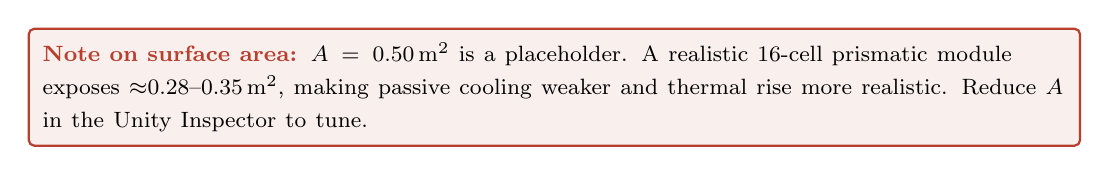
\begin{tikzpicture}
  \node[draw=warn,fill=warn!8,rounded corners=2pt,line width=0.8pt,
        text width=13.0cm,inner sep=5pt]{%
    \footnotesize\textbf{\color{warn}Note on surface area:}
    $A=0.50$\,m$^2$ is a placeholder.
    A realistic 16-cell prismatic module exposes ${\approx}0.28$--$0.35$\,m$^2$,
    making passive cooling weaker and thermal rise more realistic.
    Reduce $A$ in the Unity Inspector to tune.};
\end{tikzpicture}
\end{frame}

% =============================================================================
% 15 PIPELINE  (larger Unity box so text fits cleanly)
% =============================================================================
\begin{frame}{3D Asset \& Unity Pipeline}
\centering
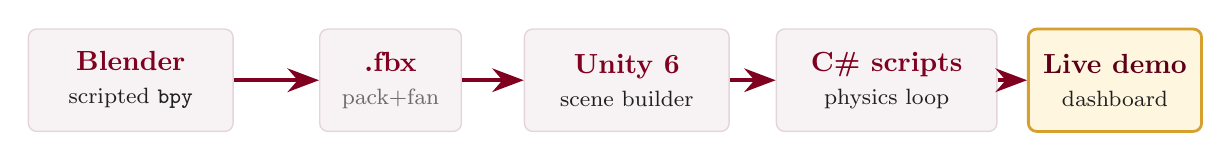
\begin{tikzpicture}[node distance=1.3cm]
  \node[card,minimum width=2.6cm,minimum height=1.3cm,align=center]
    (bl)at(0.3,0)
    {\bfseries\color{maroon}Blender\\\footnotesize\color{ink}scripted \texttt{bpy}};
  \node[card,minimum width=1.8cm,minimum height=1.3cm,align=center]
    (fbx)at(3.6,0)
    {\bfseries\color{maroon}.fbx\\\footnotesize\color{muted}pack+fan};
  \node[card,minimum width=2.6cm,minimum height=1.3cm,align=center]
    (un)at(6.6,0)
    {\bfseries\color{maroon}Unity 6\\\footnotesize\color{ink}scene builder};
  \node[card,minimum width=2.8cm,minimum height=1.3cm,align=center]
    (cs)at(9.9,0)
    {\bfseries\color{maroon}C\# scripts\\\footnotesize\color{ink}physics loop};
  \node[card,minimum width=2.2cm,minimum height=1.3cm,align=center,
        fill=accentbg,draw=accentbd,line width=1pt]
    (demo)at(12.8,0)
    {\bfseries\color{maroondk}Live demo\\\footnotesize\color{ink}dashboard};
  \draw[arrowstrong](bl)--(fbx);
  \draw[arrowstrong](fbx)--(un);
  \draw[arrowstrong](un)--(cs);
  \draw[arrowstrong](cs)--(demo);
\end{tikzpicture}

\vspace{0.25cm}
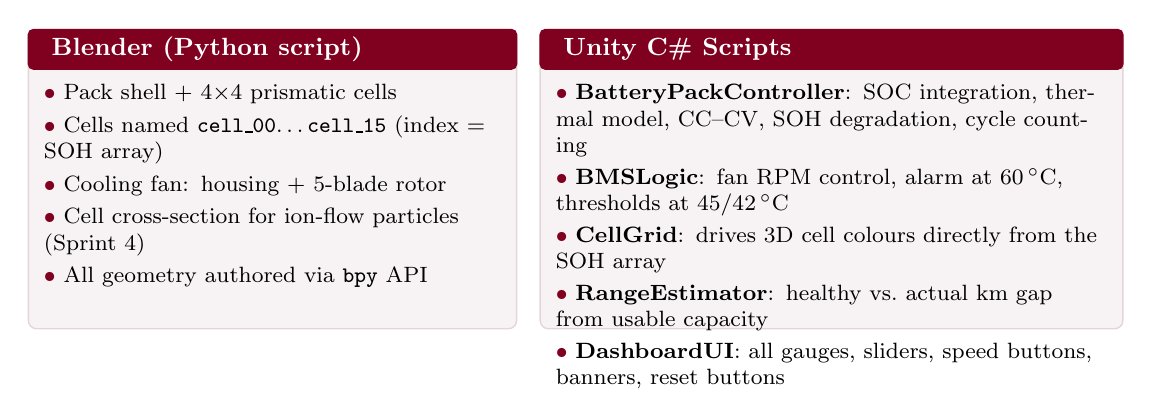
\begin{tikzpicture}
  % Blender card
  \node[card,minimum width=6.2cm,minimum height=3.8cm,
        anchor=north west](b)at(0,0){};
  \fill[maroon,rounded corners=2pt](b.north west)
    rectangle([yshift=-0.52cm]b.north east);
  \node[anchor=west,white,font=\small\bfseries]
    at([xshift=0.18cm,yshift=-0.26cm]b.north west){Blender (Python script)};
  \node[anchor=north west,text width=5.75cm,font=\footnotesize,inner sep=0]
    at([xshift=0.2cm,yshift=-0.70cm]b.north west){%
    {\color{maroon}$\bullet$}~Pack shell + 4$\times$4 prismatic cells\\[0.08cm]
    {\color{maroon}$\bullet$}~Cells named \texttt{cell\_00}\ldots\texttt{cell\_15}
      (index = SOH array)\\[0.08cm]
    {\color{maroon}$\bullet$}~Cooling fan: housing + 5-blade rotor\\[0.08cm]
    {\color{maroon}$\bullet$}~Cell cross-section for ion-flow particles (Sprint 4)\\[0.08cm]
    {\color{maroon}$\bullet$}~All geometry authored via \texttt{bpy} API};

  % Unity card — wider and taller to fit all bullets cleanly
  \node[card,minimum width=7.4cm,minimum height=3.8cm,
        anchor=north west](u)at(6.5,0){};
  \fill[maroon,rounded corners=2pt](u.north west)
    rectangle([yshift=-0.52cm]u.north east);
  \node[anchor=west,white,font=\small\bfseries]
    at([xshift=0.18cm,yshift=-0.26cm]u.north west){Unity C\# Scripts};
  \node[anchor=north west,text width=6.9cm,font=\footnotesize,inner sep=0]
    at([xshift=0.2cm,yshift=-0.70cm]u.north west){%
    {\color{maroon}$\bullet$}~\textbf{BatteryPackController}:
      SOC integration, thermal model, CC--CV, SOH degradation, cycle counting\\[0.07cm]
    {\color{maroon}$\bullet$}~\textbf{BMSLogic}:
      fan RPM control, alarm at 60\,$^\circ$C, thresholds at 45/42\,$^\circ$C\\[0.07cm]
    {\color{maroon}$\bullet$}~\textbf{CellGrid}:
      drives 3D cell colours directly from the SOH array\\[0.07cm]
    {\color{maroon}$\bullet$}~\textbf{RangeEstimator}:
      healthy vs.\ actual km gap from usable capacity\\[0.07cm]
    {\color{maroon}$\bullet$}~\textbf{DashboardUI}:
      all gauges, sliders, speed buttons, banners, reset buttons};
\end{tikzpicture}
\end{frame}

% =============================================================================
% 16 ROADMAP
% =============================================================================
\begin{frame}{Roadmap --- Sprint 3 \& Beyond}
\centering
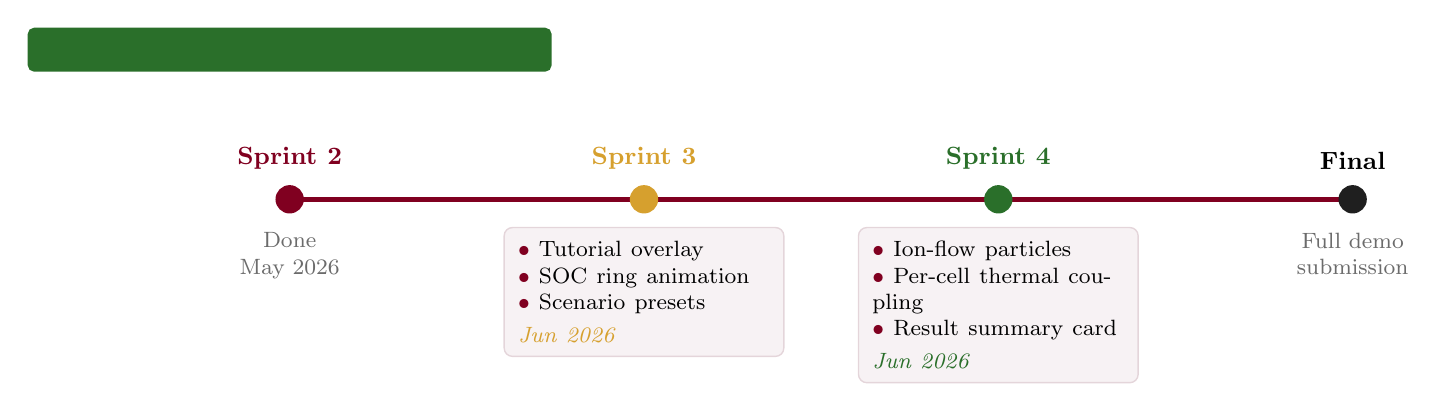
\begin{tikzpicture}
  \draw[maroon,line width=2pt](0,0)--(13.5,0);
  \fill[maroon](0,0)circle(0.18);
  \node[font=\small\bfseries,maroon,anchor=south]at(0,0.25){Sprint 2};
  \node[font=\footnotesize,muted,anchor=north,text width=2.5cm,align=center]
    at(0,-0.3){Done\\May 2026};
  \fill[accentbd](4.5,0)circle(0.18);
  \node[font=\small\bfseries,accentbd,anchor=south]at(4.5,0.25){Sprint 3};
  \node[card,anchor=north,text width=3.2cm,inner sep=5pt]at(4.5,-0.35){%
    \footnotesize
    {\color{maroon}$\bullet$}~Tutorial overlay\\
    {\color{maroon}$\bullet$}~SOC ring animation\\
    {\color{maroon}$\bullet$}~Scenario presets\\
    {\color{accentbd}\itshape Jun 2026}};
  \fill[good](9.0,0)circle(0.18);
  \node[font=\small\bfseries,good,anchor=south]at(9.0,0.25){Sprint 4};
  \node[card,anchor=north,text width=3.2cm,inner sep=5pt]at(9.0,-0.35){%
    \footnotesize
    {\color{maroon}$\bullet$}~Ion-flow particles\\
    {\color{maroon}$\bullet$}~Per-cell thermal coupling\\
    {\color{maroon}$\bullet$}~Result summary card\\
    {\color{good}\itshape Jun 2026}};
  \fill[ink](13.5,0)circle(0.18);
  \node[font=\small\bfseries,anchor=south]at(13.5,0.25){Final};
  \node[font=\footnotesize,muted,anchor=north,align=center]
    at(13.5,-0.3){Full demo\\submission};
  \node[draw=good,fill=leaf,rounded corners=2pt,line width=0.8pt,
        font=\footnotesize\bfseries,color=good,inner sep=4pt]
    at(0,1.9){$\checkmark$~Sprint 2 complete --- live demo running};
\end{tikzpicture}
\vspace{0.3cm}
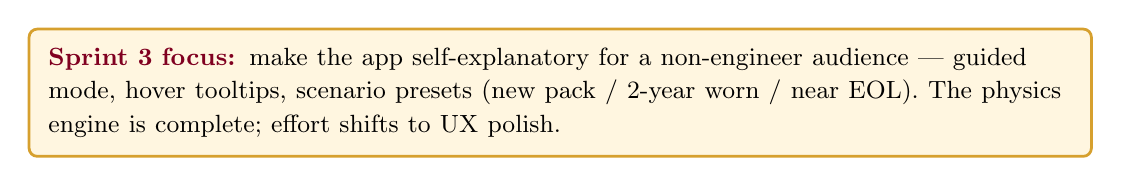
\begin{tikzpicture}
  \node[callout,text width=13.0cm,inner sep=7pt]{%
    \small\textbf{\color{maroon}Sprint 3 focus:}
    make the app self-explanatory for a non-engineer audience ---
    guided mode, hover tooltips, scenario presets
    (new pack / 2-year worn / near EOL).
    The physics engine is complete; effort shifts to UX polish.};
\end{tikzpicture}
\end{frame}

% =============================================================================
% 17 THANK YOU
% =============================================================================
\begin{frame}[plain]
\begin{tikzpicture}[overlay,remember picture]
  \fill[maroon](current page.south west)rectangle(current page.north east);
\end{tikzpicture}
\vfill\centering
{\color{white}\bfseries\Huge Thank You}\\[0.45cm]
{\color{white}\rule{2.5cm}{1.5pt}}\\[0.45cm]
{\color{white}\itshape\Large We are open for questions.}\\[0.6cm]
{\color{white}\normalsize Group 6 \quad\textbar\quad Sprint 2 \quad\textbar\quad May 2026}\\[0.3cm]
{\color{white!70}\footnotesize Live Unity demo available --- ask us to run any scenario.}
\vfill
\end{frame}

\end{document}
